\chapter{Detection and Isolation}
\label{chap:Detection}
Detecting the anomaly is a binary classification. The method implemented must therefore be able to distinguish between normal data and anomalies. There are various methods that can be implemented for this use case, however only three supervised learning methodologies and two unsupervised learning methods are implemented. The major difference between the supervised learning and the unsupervised learning methods for anomaly detection is that for supervised learning the number of anomalous samples and normal samples should be more or less the same, while with unsupervised learning the anomalous samples should be sparse. For simplicity a dataset of $n$ samples is given as 
\begin{equation}
\begin{aligned}
\mathbf{D} &= \left(\mathbf{f}_1, y_1 \right), \ldots , \left(\mathbf{f}_n, y_n \right), \\
\text{where} \qquad \mathbf{f} & \in \mathbf{R^m}. \\
\end{aligned}
\end{equation}
$\mathbf{f}$ is the point vector within the vector space, $\mathbf{R}$, with $\mathbf{m}$ dimensions, while $y$ denotes the class of the feature, which in binary classification is either $0$ or $1$.
\section{Supervised Learning}
Supervised learning is a subgroup of machine learning which is based on training algorithms from labelled data to ensure accurate predictions.

\subsection{Decision Trees}
Decision Trees and Random Forests will be implemented to perform binary classification on regular data samples and anomalous data samples. Decision Trees \cite{Reif2008} and Random Forests \cite{Shi2006, Paul2018, Primartha2018} are supervised learning algorithms that classify data based on threshold splitting. Data samples are split based on a threshold of a specific input parameter. For instance, binary classification can be performed on data samples from a satellite orbit to determine whether the satellite was in an eclipse or not. This would be done by determining whether the magnitude of the sun vector is smaller or greater than $0$. Consequently, after two splits it can be determined which data samples are within an eclipse. The Decision Tree determines this split with the classification and regression tree (CART) algorithm.

However, to split the data for the anomalies, we need to decide which input parameter will be used to make the first split, the root node. The Gini index measures the probability of a data sample being wrongly classified at a given node. This can be calculated by

\begin{equation}
GI = 1 - \sum_{i = 1}^{n}{(P_i)^2}.
\label{eq:Gini index}
\end{equation}

The operator split that produces the lowest Gini index provides the purest split and will be used as the root node. For our use case, the CART algorithm will be used to optimize the Decision Tree, which also considers the most prominent information gained to construct the Decision Tree. Figure \ref{fig:DecisionTree} is a graphical representation of the Decision Tree developed to classify anomalies. In Figure \ref{fig:DecisionTree} the \emph{samples} label provides the percentage of samples within the node with respect to the total training data samples while the \emph{value} label provides the portion of each class within the node i.e. Normal samples or Anomalous samples. The depth of a Decision Tree determines how many splits occur from the root node to the leaf node the furthest from the first split. If the depth is unspecified, the Decision Tree will split until all the data samples are perfectly split into anomalous and normal data samples. However, the larger the depth, the more biased the Decision Tree is to the training data. This depth can be altered to optimize the efficiency and accuracy of the Decision Tree.

\begin{figure*}[!hbt]
	\centering
	\def\svgwidth{16cm}
	\import{Figures/}{DecisionTree.pdf_tex}
	\caption{Decision Tree as binary classification of sun reflection. Orange nodes have more than $50\%$ normal samples, while blue nodes have more than $50\%$ anomalous samples. The darker the shade of orange or blue, the larger the percentage of the respective class.}
	\label{fig:DecisionTree}
\end{figure*}

\begin{figure}[!htb]
	\centering
	\import{Figures/TexFigures/Summary/DecisionTrees100/}{Estimation MetricPredictionWithVaryingIsolationAccuracies.pgf}
	
	\caption{Estimation Metric of Decision Trees at varying isolation percentages.}
	\label{fig:DecisionTreesWithVaryingIsolationEstimation}
\end{figure}

\begin{figure}[!htb]
	\centering
	\import{Figures/TexFigures/Summary/DecisionTrees100/}{Prediction AccuracyPredictionWithVaryingIsolationAccuracies.pgf}
	
	\caption{Prediction Accuracy of Decision Trees at varying isolation percentages.}
	\label{fig:DecisionTreesWithVaryingIsolationPrediction}
\end{figure}


It is evident in Figure \ref{fig:DecisionTree} that the most notable splits at the beginning of the tree are the moving average from the feature extraction (DMD) as well as the sun sensor and magnetometer measurements. This makes logical sense since the moving average provides the system with an extracted feature that correlates with the change in measurements. The sun reflection can also be detected on the sun sensor measurements, and changes in the control torques influences the magnetometer readings.

\subsection{Random Forests}
Random forests, (RF), is an extension of the decision tree. It generates various decision trees from the data set and provides a classification output, $\mathbf{P}$, for a new data sample, $\mathbf{D}*$, by utilizing a majority vote from all the decision trees with an individual classification output of, $\mathbf{p}_i$. RF utilizes bootstrap aggregating, $\mathbf{ba}()$, to ensure that new random data sets, $\mathbf{D}'$ with size of $n'$ is created \cite{Primartha2018, Paul2018, Shi2006}. The individual decision trees of number $k$ is then trained with Algorithm~\ref{alg: Random-Forest-training}.

\begin{algorithm}[!htb]
	\caption[Random Forest]{Training of Random Forest from Individual Decision Trees}
	\label{alg: Random-Forest-training}
	\begin{algorithmic}[1]
		\For{$i \coloneqq 1$ \textbf{to} $k$}
		\State \texttt{$\mathbf{D}_i' = \mathbf{ba}(D)$}
		\State \texttt{$\mathbf{DT_i} = \mathbf{CART}(\mathbf{D}_i')$}
		\EndFor
	\end{algorithmic}
\end{algorithm}
The classification output, $\mathbf{P}$, is then provided with Algorithm~\ref{alg: Random-Forest-prediction}.
\begin{algorithm}[!htb]
	\caption[Random Forest]{Prediction of Random Forest from Individual Decision Trees}
	\label{alg: Random-Forest-prediction}
	\begin{algorithmic}[1]
	\For{$i \coloneqq 1$ \textbf{to} $k$}
	\State \texttt{$\mathbf{p}_i = \mathbf{DT_i}(\mathbf{D}*)$}
	\EndFor
	\State $\mathbf{P} = \textbf{mode}(\mathbf{p})$
	\end{algorithmic}
\end{algorithm}

\begin{figure}[!htb]
	\centering
	\import{Figures/TexFigures/Summary/RandomForest100/}{Estimation MetricPredictionWithVaryingIsolationAccuracies.pgf}
	
	\caption{Estimation Metric of Random Forest at varying isolation percentages.}
	\label{fig:RandomForestWithVaryingIsolationEstimation}
\end{figure}

\begin{figure}[!htb]
	\centering
	\import{Figures/TexFigures/Summary/RandomForest100/}{Prediction AccuracyPredictionWithVaryingIsolationAccuracies.pgf}
	
	\caption{Prediction Accuracy of Random Forest at varying isolation percentages.}
	\label{fig:RandomForestWithVaryingIsolationPrediction}
\end{figure}

\subsection{Support Vector Machines}
A study conducted by \cite{colagrossi2022fault} implemented Support vector machines (SVM) for sensor and actuator failure detection on small satellites systems. This example as well as many other fault detection research in other fields implement SVM for anomaly detection. SVM creates a hyperplane between the feature space to increase the margin between the data samples nearest to the hyperplane from all the classes within the data \cite{hearst1998support, meyer2015support}. The hyperplane can be defined as
\begin{equation}
\mathbf{w}^T(\mathbf{x}) + b = 0
\end{equation}
where $\mathbf{w}$ is the normal vector to the hyperplane, however it is not necessarily a unit vector. This is also constrained to ensure that all vector points $\mathbf{x}_n$ are on the correct side of the hyperplane with 
\begin{equation}
\mathbf{w}^T(\mathbf{x}_i) + b \geq 1, \qquad \textbf{for all }  1 \leq i \leq n.
\end{equation}
The hyperplane in it's most simplified form is linear and divides the data into two halves based as shown in Figure~\ref{fig:SupportVectorMachinesExample}. The distance between the hyperplane and any point vector, $\mathbf{f}_i$, can be given as
\begin{equation}
d(\mathbf{x}_i) = \frac{\mathbf{w}^T(\mathbf{x}_i) + b}{\norm{\mathbf{w}}^2}
\end{equation}

\begin{figure}[!hbt]
	\centering
	\import{Figures/}{SupportVectorMachinesExample.pgf}
	\caption{Support Vector Machine Example}
	\label{fig:SupportVectorMachinesExample}
\end{figure}

For binary classification all point vectors, $\mathbf{x}_n$ will be classified into a group  . To increase the margin of between all point vectors, $\mathbf{x}_n$, and the hyperplane the minimum distance of all the point vectors and the hyperplane is required. The objective of the algorithm is therefore to maximise the minimum distance between the hyperplane and any point vector, $\mathbf{x}_i$, for all data samples $n$. This is however extended to a soft-margin optimization algorithm given as
\begin{equation}
\label{Eq-maxSVM}
\lambda \norm{\mathbf{w}}^2 + \left[\frac{1}{n} \sum_{i=1}^{n} \textbf{max} \left(0, 1 - \mathbf{w}^T\left(\mathbf{x}_i \right) + b \right) \right],
\end{equation}
where $\lambda$ increases and decreases the margin size ensuring that all training $\mathbf{x}_i$ are on the correct side of the hyperplane. An example of an algorithm used to solve the optimisation of Eq~\ref{Eq-maxSVM} is the sub-gradient descent given as
\begin{equation}
\boldsymbol{f}(\mathbf{w}, b) = \lambda \norm{\mathbf{w}}^2 + \left[\frac{1}{n} \sum_{i=1}^{n} \textbf{max} \left(0, 1 - \mathbf{w}^T\left(\mathbf{x}_i\right) + b \right) \right],
\end{equation}
where $\boldsymbol{f}$ is a convex function and can be solved with an adaptation of classic gradient descent methods. The difference is that the direction of gradient descent is that of the vector selected from the function's sub-gradient. With this implementation the hyperplane can divide two groups as shown given in Figure~\ref{fig:SupportVectorMachinesExample}. The vector points within the margin size and with the additional black circle in Figure~\ref{fig:SupportVectorMachinesExample} are called the support vectors since these vector points are the minimum distance from the hyperplane and influence Eq~\ref{Eq-maxSVM}.

The linear hyperplane is not always feasible, since certain data samples cannot be divided with a single line. There are two solutions to this problem. The first is to increase the dimension size, $\mathbf{m}$, of $\mathbf{R^m}$. For instance increasing $m$ from $2$ to $3$ with 
\begin{equation}
\mathbf{x}[2] = \sqrt{\mathbf{x}[0]^2 + \mathbf{x}[1]}
\end{equation}
provides a higher dimension for the split of the data. This can be implemented with any equation for increasing $\mathbf{m}$. An example of this can be seen by increasing $m$ from $2$ in Figure~\ref{fig:SupportVectorMachinesExample} to $3$in Figure~\ref{fig:SupportVectorMachines3DExample} by adding another feature from the data. A $3$D hyperplane can now divide the data into two separate groups.

\begin{figure}[!hbt]
	\centering
	\import{Figures/}{SupportVectorMachines3DExample.pgf}
	\caption{Support Vector Machine Higher Dimension Example}
	\label{fig:SupportVectorMachines3DExample}
\end{figure}

Another method to divide the data into different classes is by changing the kernel from linear to non-linear kernels such as a polynomial kernel. A linear kernel is given as 
\begin{equation}
\mathbf{K}\left(x_i,x_j \right) = x_i^Tx_j+ \mathbf{C},
\end{equation}
whereas a poynomial kernel is given as
\begin{equation}
\mathbf{K}\left(x_i,x_j \right) = \left(\gamma x_i^Tx_j + r \right)^d, \qquad \gamma > 0.
\end{equation}
This is provided with the example of a polynomial division of the data shown in Figure~\ref{fig:SupportVectorMachinesExample} with a polynomial fit of the $3^{\text{rd}}$ degree as shown in Figure~\ref{fig:SupportVectorMachinesExamplePoly}. The kernel will depend on the nature of the data and the relationship between the different features. This is therefore an iterative process to decide the kernel unless available opensource algorithms are used to determine which kernel structure is the best suited for the current dataset.

\begin{figure}[!hbt]
	\centering
	\import{Figures/}{SupportVectorMachinesExamplePoly.pgf}
	\caption{Support Vector Machine Polynomial Example}
	\label{fig:SupportVectorMachinesExamplePoly}
\end{figure}

\begin{figure}[!htb]
	\centering
	\import{Figures/TexFigures/Summary/SVM/}{Estimation MetricPredictionWithVaryingIsolationAccuracies.pgf}
	
	\caption{Estimation Metric of Support Vector Machines at varying isolation percentages.}
	\label{fig:SVMWithVaryingIsolationEstimation}
\end{figure}

\begin{figure}[!htb]
	\centering
	\import{Figures/TexFigures/Summary/SVM/}{Prediction AccuracyPredictionWithVaryingIsolationAccuracies.pgf}
	
	\caption{Prediction Accuracy of Support Vector Machines at varying isolation percentages.}
	\label{fig:SVMWithVaryingIsolationPrediction}
\end{figure}

\section{Unsupervised Learning}
Supervised learning is a subgroup of machine learning which is based on unlabelled data. Local Outlier factor as discussed in Section~\ref{section:OutlierFactor} can also be implemented as an unsupervised learning method.

\subsection{Isolation Forests}
This unsupervised learning method is based on the principle of isolating data points by slicing the data with random conditions \cite{TonyLiu2008}. The data is randomly split into specified sample sizes with a randomly selected dimension and a randomly selected cut-off value. For each sample size the data must be split until each data point within the sample is isolated from all other data points. Training of a single tree is completed when all the data points are isolated and this training must be repeated for all the data samples, however many are predefined. 

The distance measured from the first split the \emph{tree top} to the isolated data point is used to determine whether a data point is anomalous or not \cite{Hariri2021}. The logical reasoning for support of this algorithm is that data points which are non-anomalous will be more closely related and hence have more splits to separate the data points until isolation is achieved. Therefore, the distance from the tree top for non-anomalous data points will be longer than anomalous data points which will have a shorter distance from the tree top. Therefore non-anomalous data points are closer to the \emph{root}. 

Figure~\ref{Figure-Isolation_Forest} demonstrates the splitting of the data points until isolated. Each split or \emph{branch} only splits the data into two groups. After training multiple trees, a single data point is "sent through the forest" and the distance from the tree top for each tree is calculated and the average of all the trees are used to calculated the average distance for the data point. Using a threshold for the distance, the data point is classified as anomalous or not.

\begin{figure}[h!tb]
	\centering
	
	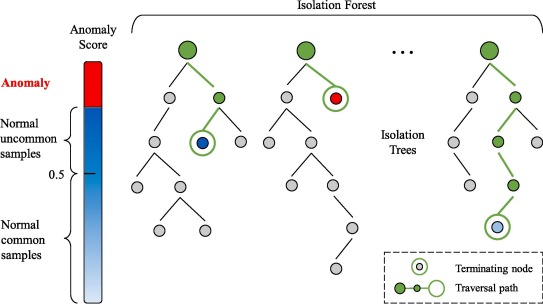
\includegraphics[width=10cm]{fig/Isolation_Forests} % not necessary to give extension - now you can shift between compiling to ps or to pdf without any problems
	
	\caption[Isolation Forest]{Isolation Forests \cite{Chen2020}}
	\label{Figure-Isolation_Forest} 
\end{figure}

An example of a trained isolation forest is provided in Figure~\ref{fig:IsolationForest}. The samples in white are the training samples of which all are considered normal data. Therefore the tree is constructed and the branches are created until all the data samples in the training data set are divided into individual nodes. Thereafter, the new data set is classified and is evident that data samples far removed from the normal training samples are isolated within the anomaly threshold and are therefore considered anomalous (depicted as red). \textbf{TODO: Ensure that isolation forest is done trained with no anomaly samples}.
\begin{figure}[!hbt]
	\centering
	\import{Figures/}{IsolationForest.pgf}
	\caption{Isolation Forest}
	\label{fig:IsolationForest}
\end{figure}

The anomaly score is calculated as
\begin{equation}
	s(x,n) = 2^{-E(h(x))/c(n)},
	\label{Eq-Isolation_anomaly}
\end{equation}
where $E(h(x))$ is the average value of the distance measured from the tree top for a single data point in all the trees \cite{Hariri2021} and $n$ is the size of a data sample used to train a single tree. For the distance to be normalized, $c(n)$ --- the mean distance from the tree top in an unsuccessful search in a \emph{Binary Search Tree} (BST) --- is used and is calculated as 
\begin{equation}
	c(n) = 2H(n-1) - \frac{2(n-1)}{n}.
	\label{Eq-normalizing_isolation}
\end{equation}
$H(i)$ in Eq~\ref{Eq-normalizing_isolation} is the harmonic number and is estimated with Euler's constant as 
\begin{equation}
	H(i) \approx \ln(i) + 0.5772156649.
	\label{Eq-H_i}
\end{equation}
Isolation Forests, however have multiple issues, since it splits data in rectangles as seen in Figure~\ref{fig:IsolationForest} and Figure~\ref{Figure-ExtendedvsNormal_first}. This is due to the slicing algorithm selecting a feature, $x$ and a cut-off value, $v$. Consequently, the data is either split vertically or horizontally --- if seen as a two dimensional dataset. This split method is unable to categorise complex data structures. These issues however are addressed by \cite{Hariri2021} and led to the \emph{Extended Isolation Forest} algorithm.

The extended isolation forest algorithm generalises the isolation forest algorithm by applying a slope to each slice. Data points are therefore divided into two groups depending on the "side" of the plane or slice as seen in Figure~\ref{Figure-ExtendedvsNormal_second}.

\begin{figure}[h!tb]
	\centering
	
	\subfloat[][Isolation Forest Slicing example]{
		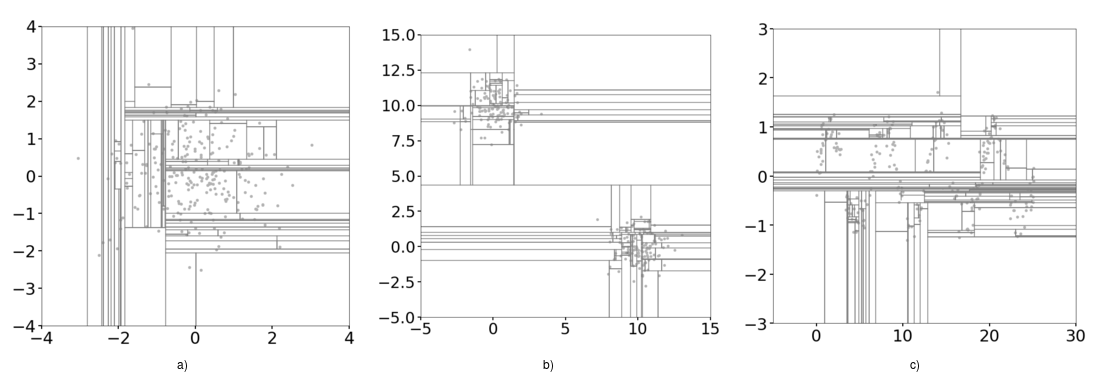
\includegraphics[trim = 0 0 725 0, clip = true, width=7cm]{fig/Isolation_forest_slicing}
		\label{Figure-ExtendedvsNormal_first}
	}
	\quad
	\subfloat[][Extended Isolation Forest Slicing example]{
		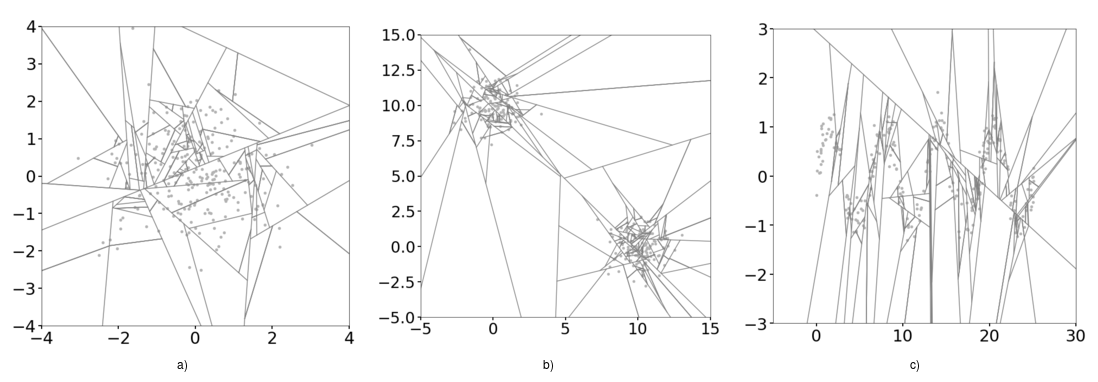
\includegraphics[trim = 0 0 725 0, clip=true,width=7cm]{fig/Extended_Isolation_forest_slicing}
		\label{Figure-ExtendedvsNormal_second}
	}]\
	\caption[Slicing of Isolation Forest]{The slicing of Isolation Forest vs Extended Isolation Forest}
	\label{Figure-ExtendedvsNormal}
\end{figure}

It is evident that applying an angle of $0\degree$ to all the slices the general algorithm of the extended isolation forest produces the standard isolation forest algorithm where planes or slices are perpendicular to the axis of the randomly selected feature, $x$.

\begin{figure}[!htb]
	\centering
	\import{Figures/TexFigures/Summary/IsolationForest/}{Estimation MetricPredictionWithVaryingIsolationAccuracies.pgf}
	
	\caption{Estimation Metric of Isolation Forest at varying isolation percentages.}
	\label{fig:IsolationForestWithVaryingIsolationEstimation}
\end{figure}

\begin{figure}[!htb]
	\centering
	\import{Figures/TexFigures/Summary/IsolationForest/}{Prediction AccuracyPredictionWithVaryingIsolationAccuracies.pgf}
	
	\caption{Prediction Accuracy of Isolation Forest at varying isolation percentages.}
	\label{fig:IsolationForestWithVaryingIsolationPrediction}
\end{figure}

\section{Local Outlier Factor}
\begin{figure}[!htb]
	\centering
	\import{Figures/TexFigures/Summary/LOF/}{Estimation MetricPredictionWithVaryingIsolationAccuracies.pgf}
	
	\caption{Estimation Metric of Local Outlier Factor at varying isolation percentages.}
	\label{fig:LOFWithVaryingIsolationEstimation}
\end{figure}

\begin{figure}[!htb]
	\centering
	\import{Figures/TexFigures/Summary/LOF/}{Prediction AccuracyPredictionWithVaryingIsolationAccuracies.pgf}
	
	\caption{Prediction Accuracy of Local Outlier Factor at varying isolation percentages.}
	\label{fig:LOFWithVaryingIsolationPrediction}
\end{figure}

\section{Comparison of Detection Methods}
\begin{figure}[!htb]
	\centering
	\import{Figures/TexFigures/Summary/100.0/}{Estimation MetricPerfectIsolationComparePredictions.pgf}
	
	\caption{Comparison of Estimation Metric of Detection Methods with an isolation accuracy of $100\%$.}
	\label{fig:DetectionMethodsWithPerfectIsolation}
\end{figure}

\section{Summary}
For the detection of anomalies different binary classification methods are discussed. This includes supervised learning methods such as decision trees, random forests and support vector machines as well as unsupervised learning methods such as isolation forests and local outlier factor which is only discussed in Section~\ref{section:OutlierFactor}. Both supervised and unsupervised learning methods for detection only provide a binary split between anomalous and normal data points, however supervised learning methods can also be implemented for isolation, multi-class classification.